\documentclass[12pt,a4paper]{report}
\usepackage[utf8]{inputenc}
\usepackage{cite}
\usepackage{float}
\usepackage{csquotes}
\usepackage[english]{babel}
\usepackage{multirow}
\usepackage[normalem]{ulem}
\useunder{\uline}{\ul}{}
\usepackage{hyperref}
\usepackage{graphicx}
\usepackage[T1]{fontenc}
\usepackage{listings}
\usepackage{xcolor}

\lstdefinestyle{bashstyle}{
    language=bash,
    basicstyle=\small\ttfamily,
    backgroundcolor=\color{gray!10},
    frame=tb,
    framerule=0pt,
    aboveskip=3mm,
    belowskip=3mm,
    showstringspaces=false,
    columns=flexible,
    numbers=none,
    keywordstyle=\color{blue},
    commentstyle=\color{gray},
    stringstyle=\color{green!60!black},
    breaklines=true,
    breakatwhitespace=true,
    tabsize=4
}

\title{Verificarea rețelelor neuronale folosind cGAN}
\author{Laptedulce Anastasia \\ Morariu Ioana-Alexandra \\ Romaneț Rareș  \\ Domșa Emanuel \\ Diaconu Laura}

\date{\href{https://github.com/IoanaMorariu/verificare_formala}{GitHub}}

\begin{document}
\maketitle
\begin{abstract}
\hspace{0.5 cm} In this paper we explored and tested the use of Conditional Generative Adversarial Networks and it's features in the context of image recognition tasks. For testing matters we use the cGAN benchmark from VNNComp 2023. The paper includes description of the above mentioned benchmark, details of configuration and running alpha\textunderscore beta\textunderscore crown tool and a short interpretation of the obtained results.


\end{abstract}


%%%%%%%%%%%%%%%%%%%%%%%%%%%%%%%%%%%%%INTRODUCERE%%%%%%%%%%%%%%%%%%%%%%%%%%%%%%%%%%%%
\section*{Introducere}
\hspace{0.5 cm} Verificarea rețelelor neuronale este un proces esențial în dezvoltarea și implementarea acestor modele avansate. Această practică reprezintă un pilon fundamental din mai multe motive cheie.

În primul rând, corectitudinea și fiabilitatea rețelelor neuronale sunt imperative. Acestea sunt utilizate într-o varietate de domenii, de la medicină și tehnologie la securitate cibernetică și vehicule autonome. Verificarea asigură că aceste rețele operează conform așteptărilor, furnizând rezultate precise și de încredere într-o gamă largă de scenarii.

Siguranța este un alt aspect crucial. În aplicații critice, cum ar fi cele medicale sau cele legate de siguranța vehiculelor, erorile în funcționarea rețelelor neuronale pot avea consecințe grave. Verificarea acestora este vitală pentru a identifica și a remedia potențialele vulnerabilități care ar putea compromite siguranța sistemelor.

De asemenea, verificarea rețelelor neuronale ajută la prevenirea bias-ului și discriminării. Aceste rețele pot fi susceptibile la prejudecăți încorporate din datele de antrenament. Prin testare și evaluare riguroasă, se poate identifica și corecta aceste bias-uri pentru a asigura obiectivitate și echitate în rezultatele furnizate.
%%%%%%%%%%%%%%%%%%%%%%%%%%%%%%%%%%%%%INTRODUCERE%%%%%%%%%%%%%%%%%%%%%%%%%%%%%%%%%%%%

%%%%%%%%%%%%%%%%%%%%%%%%%%%%%%%%%%%%%Descriere data set%%%%%%%%%%%%%%%%%%%%%%%%%%%%%
\section*{Descrierea data set-ului cGAN}
\hspace{0.5 cm} În contextul verificării rețelelor neuronale, un benchmark este constituit dintr-o serie de modele neurale testate și specificațiile riguroase ce trebuie satisfăcute pentru a valida corectitudinea și securitatea acestora. 

Modelul neuronal este reprezentat sub forma fișierelor în format .onnx. Aceste fișiere cuprind detaliile arhitecturii modelului, precum straturile rețelei neuronale și parametrii, însă nu includ datele reale de antrenament.

Specificările care sunt supuse verificării sunt reprezentate printr-un set de fișiere în format .vnnlib, care conțin informații esențiale despre rețeaua neuronală. Aceste detalii includ dimensiunile stratului de intrare și de ieșire, precum și intervalul sau domeniul de valori admise pentru activările neuronale.

Benchmark-ul utilizat testează un model deosebit de reațea neuronală care se numește rețea adversară generativă condiționată. Pentru o întelegere mai bună a celui din urmă vom descrie mai întâi ce este o rețea neurală adversară generativă.

\subsection*{GAN}
 \hspace{0.5 cm} Este un model neuronal mai special \cite{GAN} a cărui concept poate fi reprezentat ca un joc între două rețele neuronale distincte adversare sau, altfel spus, între doi jucători. Primul jucator este numit generator, iar al doilea discriminator. 
 
 Rolul generatorului este de a genera date false, bazate pe datele de intrare, care să pară cât mai reale. Generatorul are scopul de a păcăli pe al doilea jucător - discriminantorul. 
 
 Scopul celui de-al doilea jucator este de a determina ce imagini sunt reale și care sunt false, adica realizate de generator. Dacă discriminatorul interpretează corect atunci primește feedback pozitiv, dacă interpretează greșit atunci primește feedback negativ. Discriminatorul are  acces la datele de ce ies din generator, dar si la datele de antrenament.

\begin{figure}[ht]
\centering
{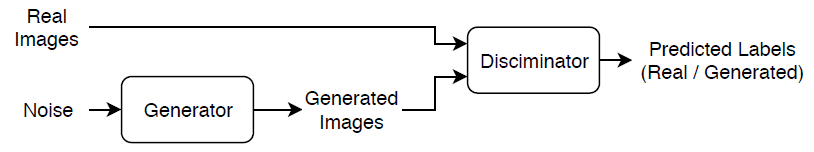
\includegraphics[width=10cm]{imagini/GANarch.png}}
\caption{Mod de lucru al GAN}
\label{modDeLucruGAN}
\end{figure}

Ambii jucători învață și se îmbunătățesc în timp. Generatorul devine mai bun în a crea falsuri convingătoare, iar discriminatorul își îmbunătățește capacitatea de a spune dacă ceva este autentic. De-a lungul timpului, rețeaua ajunge într-un punct în care datele produse de generator vor arăta aproape imposibil de distins de datele din lumea reală.



\subsection*{cGAN}
\hspace{0.5 cm} cGAN, prescurtare de la Conditional Generative Adversarial Networks \cite{CGAN}, ghidează procesul de creare a datelor prin încorporarea unor etichete specificice în GAN. Rețele adversare - generatorul și discriminatorul - se orientează după aceste etichete. 

Generatorul utilizează etichetele pentru a creea date false care imită datele reale și respectă condiția setată. Și la fel ca în modelul GAN, discriminatorul va distinge între datele falsificate produse de generator și datele autentice corespunzătoare condiției date.
\newpage

\begin{figure}[ht]
\centering
{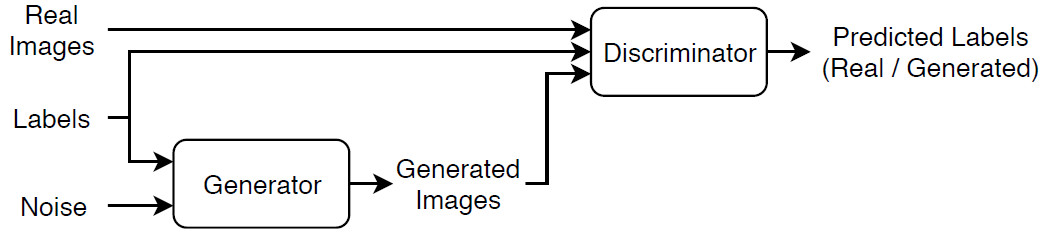
\includegraphics[width=10cm]{imagini/cGANarch.png}}
\caption{Mod de lucru al cGAN}
\label{modDeLucrucGAN}
\end{figure}



De exemplu, să presupunem că ați folosit un spectru larg de imagini cu flori pentru a antrena un GAN capabil să producă imagini false cu flori. Deși puteți folosi modelul dvs. pentru a genera o imagine a unei flori aleatorii, nu îi puteți instrui să creeze o imagine a, de exemplu, a unei lalele sau a unei floarea soarelui.

GAN condiționat (cGAN) ne permite să condiționăm rețeaua cu informații suplimentare, cum ar fi etichetele de clasă. Înseamnă că în timpul antrenamentului, transmitem imagini în rețea cu etichetele lor reale (trandafir, lalele, floarea soarelui etc.) pentru ca aceasta să învețe diferența dintre ele. În acest fel, obținem capacitatea de a cere modelului nostru să genereze imagini cu anumite flori.


\subsection*{cGAN benchmark din vnncomp2023}
Obiectivul \cite{vnncomp2023Chat} modelului neuronal din benchmark-ul cGAN din competiția vnncomp2023 este de a genera imagini ale camerei care conțin un obstacol al vehiculului situat la o anumită distanță în fața vehiculului ego, unde distanța este controlată de condiția distanței de intrare. În figura \ref{imaginiGenerate} sunt ilustrate exemple de imagini create de generatorul din cadrul retelei neurale.

\begin{figure}[ht]
\centering
{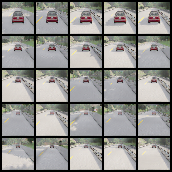
\includegraphics[width=5.75cm]{imagini/obstacle.png}}
\caption{Imagini generate}
\label{imaginiGenerate}
\end{figure}

Generatorul primește două intrări:
\begin{itemize}
\item o condiție de distanță (1-d scalar), între 0 - 1(normalizat de la 0m la 30m). De exemplu, dacă condiția de distanță este 0,5, înseamnă că va fi generată o imagine ce are obstacolul la 15m in fața vehiculului ego.
\item un vector de zgomot care controlează mediul (vector 4-d)
\end{itemize}

Ca și rezultat genratorul returnează o imagine generată.


Discriminatorul consideră imaginea returnată de generator ca și data de intrare și emite ca rezultat urmatoarele:
\begin{itemize}
\item un scor real/fals (1-d scalar), adică dacă trebuie să prezică dacă imaginea a fost realizată de generator sau nu
\item o distanță prezisă (1-d scalar), distanță estimată de discriminant dintre vehiculul ego și vehiculul obstacol
\end{itemize}

\begin{figure}[ht]
\centering
{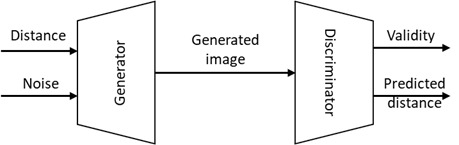
\includegraphics[width=8.5cm]{imagini/cganbench.jpeg}}
\caption{Mod de lucru cGAN benchmark}
\label{cganbench}
\end{figure}

Pentru verificare, am putea combina aceste două componente împreună și am putea stabili specificații de verificare adecvate pentru distanța de intrare, zgomotul de intrare și distanța estimată.


%%%%%%%%%%%%%%%%%%%%%%%%%%%%%%%%%%%%%Descriere data set%%%%%%%%%%%%%%%%%%%%%%%%%%%%%

%%%%%%%%%%%%%%%%%%%%%%%%%%%%%%%%%%%%%Instalarea instrumentelor%%%%%%%%%%%%%%%%%%%%%%
\section*{Configurare alpha\textunderscore beta\textunderscore crown}
\hspace{0.5 cm}
Pentru rularea benchmark-ului cGan am ales ca și tool-uri  alpha\textunderscore beta\textunderscore crown si NeuralSAT, verificând prima dată cu atenție dacă acestea au putut rula setul de date, figura \ref{cGan_gr}. Am facut această alegere deoarece am dorit o comparație dintre primul tool care a obțiunut un timp de verificare mai eficient, iar cel de al doilea care a obținut cel mai ineficient timp de verificare.

\begin{figure}[ht]
\centering
{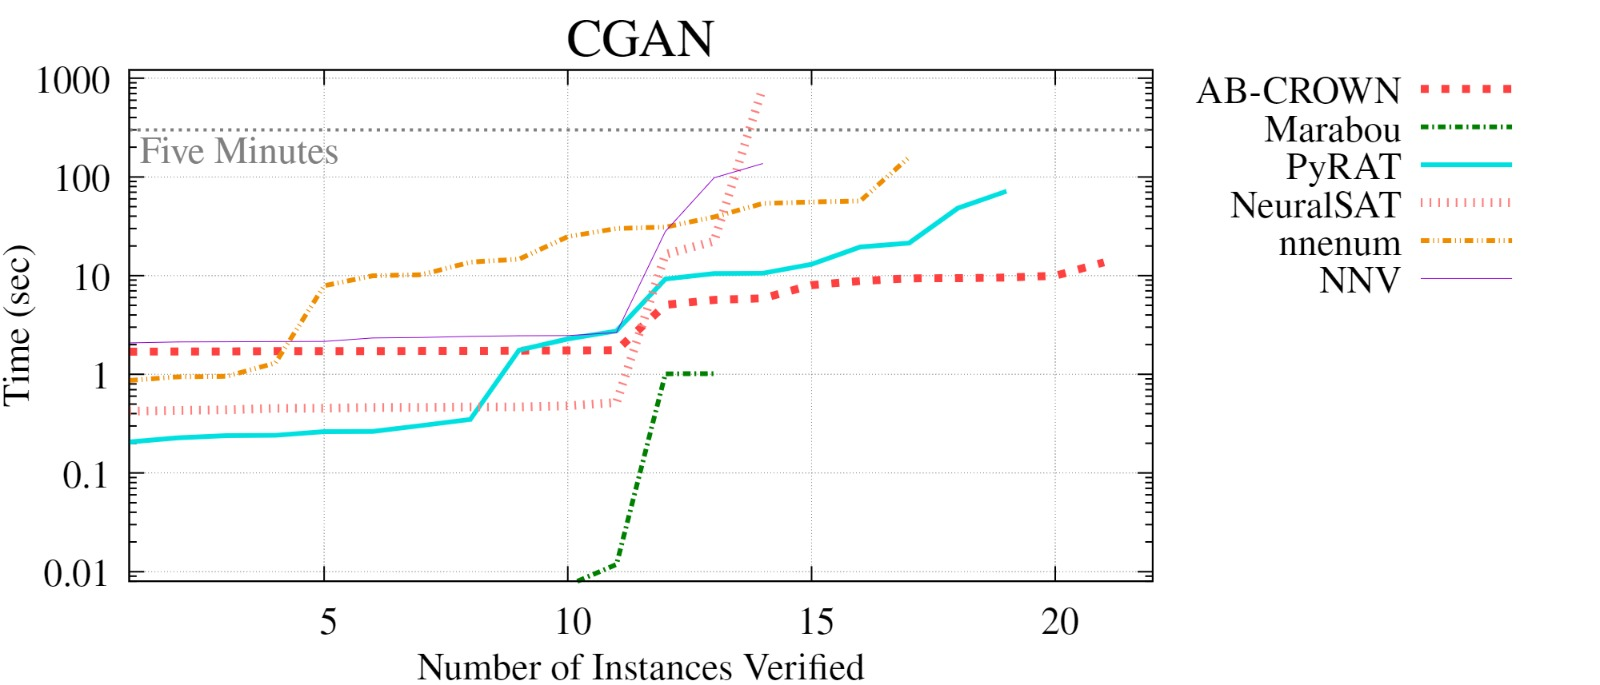
\includegraphics[width=12cm]{imagini/cGan_grafic.jpg}}
\caption{Rezultatele rulării tool-urilor pentru benchmark-ul cGan}
\label{cGan_gr}
\end{figure}

Alpha\textunderscore beta\textunderscore CROWN a fost testat pe Python 3.11, sistemul de operare utilizat a fost  Ubuntu 20.04 prin Windows Subsystem for Linux (WSL) pe Windows 10, folosind un GPU de laptop NVIDIA GeForce RTX 3060.  A fost instalat într-un mediu miniconda. În urmatorii pasi se va explica cum a fost facută instalarea și rularea tool-ului.


\subsection*{Pai de Instalare:}

\begin{enumerate}
  \item Instalarea Miniconda a fost realizată prin linia de comandă (bash) cu următorii pași:
  \begin{lstlisting}[style=bashstyle]
    mkdir -p ~/miniconda3
    wget https://repo.anaconda.com/miniconda/Miniconda3-
    latest-Linux-x86_64.sh -O ~/miniconda3/miniconda.sh
    bash ~/miniconda3/miniconda.sh -b -u -p ~/miniconda3
    rm -rf ~/miniconda3/miniconda.sh
    ~/miniconda3/bin/conda init bash
   \end{lstlisting}
  
  \item Clonarea repository-ului de la adresa \cite{crownrepository}:
    \begin{lstlisting}[style=bashstyle]
    git clone --recursive https://github.com/Verified-
    Intelligence/alpha-beta-CROWN.git
   \end{lstlisting}
  
  \item Clonarea submodulului \texttt{auto\_Lirpa} în interiorul directorului \texttt{alpha-beta-CROWN}:
    \begin{lstlisting}[style=bashstyle]
    git clone https://github.com/Verified-
    Intelligence/auto_LiRPA.git alpha-beta-CROWN/auto_LiRPA
   \end{lstlisting}
  
  \item Configurarea mediului Conda:
    \begin{lstlisting}[style=bashstyle]
    conda deactivate; conda env remove --name alpha-beta-crown
    conda env create -f complete_verifier/environment.yaml --name alpha-beta-crown
    conda activate alpha-beta-crown
   \end{lstlisting}
  
  \item Crearea directorului \texttt{vnncomp2023\_benchmarks} și clonarea repository-ului \cite{cganrepository} în interiorul acestuia. Modificarea \textbf{root path-ului} în fișierul \texttt{cgan.yaml} conform locației reale a directorului \texttt{cgan}.
  
  \item Rularea verificatorului:
  \begin{lstlisting}[style=bashstyle]
    python abcrown.py --config exp_configs/vnncomp23/cgan.yaml
  \end{lstlisting}
  
  \item Pentru a rezolva eroarea legată de \texttt{libcudnn\_cnn\_infer.so.8}, adăugarea următoarei linii în \texttt{.bashrc}:
  \begin{lstlisting}[style=bashstyle]
    export LD_LIBRARY_PATH=/usr/lib/wsl/lib:$LD_LIBRARY_PATH
  \end{lstlisting}
  
  \item Rerularea comenzii și salvarea rezultatelor în \texttt{results.txt}:
  \begin{lstlisting}[style=bashstyle]
    python abcrown.py --config exp_configs/vnncomp23/cgan.yaml > results.txt
  \end{lstlisting}
\end{enumerate}

Cel mai dificil pas a fost remedierea erorii legate de libraria libcudnn\textunderscore cnn\textunderscore infer.so.8., fiind si pasul care a durat cel mai mult timp. Am rezolvat aceasta eroare folosind multiple sugestii gasite pe diferite platforme online \cite{bashrcfix}.
%%%%%%%%%%%%%%%%%%%%%%%%%%%%%%%%%%%%%Instalarea instrumentelor%%%%%%%%%%%%%%%%%%%%%%

%%%%%%%%%%%%%%%%%%%%%%%%%%%%%%%%%%%%%Rularea%%%%%%%%%%%%%%%%%%%%%%
\section*{Interpretare rezultate}
\hspace{0.5 cm} Rezultatele obținute după rularea toolului alpha\textunderscore beta\textunderscore crown pe benchmark-ul cGAN au fost sub forma unui stream în consolă, dupa cum se vede în figura \ref{streamConsola}.

\begin{figure}[ht]
\centering
{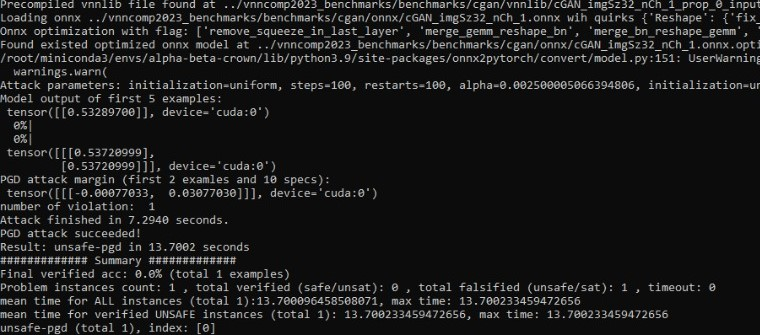
\includegraphics[width=15cm]{imagini/streamConsola.jpeg}}
\caption{Rezultat stream consola}
\label{streamConsola}
\end{figure}

Pentru a putea interpreta datele rezultate le-am clasificat manual într-un fișier excel. Câpurile de tabel sunt urmatoarele: 
\begin{itemize}
\item benchmark(benchmark-ul pentru care avem înregistrate rezultatele)

\item model\textunderscore neuronal(fișierul ONNX pentru care a rulat tool-ul)

\item specificații(fieșierul VNNLIB pentru care a rulat tool-ul)

\item rezultat(poate avea valori sat/unsat; sat înseamnă că modelul indeplinește condițiile din fișierul VNNLIB, adică distanța aproximată de discriminator, este aceeași cu distanța pe care a primit-o generator-ul ca și data de intrare; unsat înseamnă că discriminatorul nu a reușit să facă o aproximare corectă)

\item timp\textunderscore de\textunderscore verificare(timpul de rulare a fișierului ONNX pentru specificatiile din fișierul VNNLIB, exprimat în secunde). 
\end{itemize}

\href{https://docs.google.com/spreadsheets/d/1kSxunni8qgQLT6ZkCRWvSO2VMy2Hz7qA/edit#gid=1476783028}{Aici} se pot vedea rezultatele pe care le-am obținut.
Pentru a ne verifica corectitudinea rezultatelor obținute, am facut o analiză comparativă între fișierul obținut la rularea noastră, \href{https://docs.google.com/spreadsheets/d/1kSxunni8qgQLT6ZkCRWvSO2VMy2Hz7qA/edit#gid=1476783028}{aici}, și cel obținut din competiție, \href{https://drive.google.com/file/d/1XolWcngRIGwjblvrm2a5FD2AqH8fVWgt/view?usp=drive_link}{aici}. 


Am observat că pentru fiecare intrare, în ambele fișiere, s-a obținut același rezultat(sat/unsat). O diferență dintre cele două fișiere o constituie coloana ce reprezinta timpul de verificare. Am remarcat că în fișierul obținut de noi, timpul de verificare înregistrat este mai mic cu aproximativ 3 secunde pentru intrările unde rezultatul este satisfiabil. În schimb, pentru intrările cu rezultat nesatisfiabil timpul de verificare este considerabil mai mare.
%%%%%%%%%%%%%%%%%%%%%%%%%%%%%%%%%%%%Rularea%%%%%%%%%%%%%%%%%%%%%%

%%%%%%%%%%%%%%%%%%%%%%%%%%%%%%%%%%%%%Rularea%%%%%%%%%%%%%%%%%%%%%%
\section*{Concluzii}
\hspace{0.5 cm}
În această lucrare, am analizat în detaliu benchmark-ul cGAN din cadrul competiției VNN-Comp2023. Am descris pașii de instalare și rulare a instrumentelor alpha-beta-CROWN și NeuralSAT. Ulterior, am interpretarea rezultatele obținute în urma rulării. Aceste acțiuni au avut ca scop analizarea performanței și funcționării rețelelor neuronale.

Instrumentele folosite au fost dezvoltate special pentru verificarea formală a corectitudinii rețelelor neuronale. Prin intermediul rulării tool-urilor pe setul cGAN, s-a evaluat capacitatea rețelelor, din cadrul benchmark-ului, de a se alinia cu condițiile de intrare specificate în fișierele .vnnlib.

Rezultatele în urmă rulării, au fost extrase în tabele pentru a facilita compararea cu rezultatele din cadrul competiției. În compararea rezultatelor noastre cu cele din competiție, s-a observat o aliniere în ceea ce privește rezultatele satisfiabile și nesatisfiabile. Diferențe au existat, în schimb, la timpii necesari pentru verificare. Spre final, am menționat despre eficiența utilizării cGAN în contextul recunoașterii imaginilor.
%%%%%%%%%%%%%%%%%%%%%%%%%%%%%%%%%%%%Rularea%%%%%%%%%%%%%%%%%%%%%%

\bibliography{mybib}
\bibliographystyle{IEEEtran}
\bibliographystyle{alpha}
\addcontentsline{toc}{chapter}{Bibliography}

\end{document}
